\section{Evaluation}
\label{sec:pytorch_direct_evaluation}
This section evaluates PyTorch-Direct performance using a well-defined microbenchmark and end-to-end GNN training.
Using the microbenchmark, we demonstrate that (1) PyTorch-Direct is faster than the baseline PyTorch approach in accessing features from the GPU under different combinations of data sizes and systems and (2) the effectiveness of our optimized memory alignment mechanism.
In GNN training, we show the benefit of using PyTorch-Direct for faster training.

\subsection{Evaluation Setup}
\begin{table}[]
\centering
                \begin{tabular}{llcccc}
                    \toprule
                    Abbv.   & Dataset             & \#Features & Size  & \#Node & \#Edge \\
                    \midrule
                    reddit  & reddit              & 602     & 561MB & 233.0K & 11.6M  \\
                    product & ogbn-products       & 100     & 960MB & 2.4M   & 61.9M  \\
                    twit    & twitter7            & 343     & 57 GB  & 41.7M  & 1.5B   \\
                    sk      & sk-2005             & 293     & 59 GB  & 50.6M  & 1.9B   \\
                    paper   & ogbn-papers100M     & 128     & 57 GB  & 111.1M & 1.6B   \\
                    wiki    & wikipedia\_link\_en & 800     & 44 GB  & 13.6M  & 437.2M \\
                    \bottomrule
                \end{tabular}
    \caption{Datasets for GNN training, their characteristics, and abbreviations (abbv.) used in the text.}
    \label{tab:pydarxiv_datasets}
\end{table}


\noindent\textbf{Datasets.} The datasets we use for the GNN training evaluation are shown in Table~\ref{tab:pydarxiv_datasets}.
For the sk-2005~\cite{BoVWFI}, twitter7~\cite{Kwak10www}, and wikipedia\_link\_en~\cite{konect} datasets, we have created them from existing real-world graphs but with synthetic feature values just for the purpose of training time evaluation.
Datasets reddit~\cite{hamilton2017inductive}, ogbn-products, and ogbn-papers100M~\cite{huOpenGraphBenchmark2021} are commonly used datasets in the field for comparing the training accuracies between different GNN architectures.


\noindent\textbf{Test System.} The platforms we have used for the evaluation are described in Table~\ref{tab:hardware}.
We use NVIDIA 450.51.05 driver and CUDA 10.2 on the evaluation platforms.
System2 and System3 configurations are only used in Section~\ref{sec.evaluation.microbenchmarkI}.

\begin{table}[]
\centering
            \begin{tabular}{ccl}
                \toprule
                Config                   & Type & \multicolumn{1}{c}{Specifications} \\
                \midrule
                System1                  & CPU  & AMD Threadripper 3960X 24C/48T    \\
                (Primary)                & GPU  & NVIDIA TITAN Xp 12 GB              \\
                \midrule
                \multirow{2}{*}{System2} & CPU  & Dual Intel Xeon Gold 6230 40C/80T \\
                                         & GPU  & NVIDIA Tesla V100 16 GB            \\
                \midrule
                \multirow{2}{*}{System3} & CPU  & Intel i7-8700K 6C/12T             \\
                                         & GPU  & NVIDIA GTX 1660 6 GB               \\
                \bottomrule
            \end{tabular}
    \caption{Evaluation platforms. \kwc{The number of cores (C) and threads (T) of CPUs are listed in the specifications column.}}
    \label{tab:hardware}
\end{table}


\noindent\textbf{Microbenchmark.} We would like to answer the following questions with the microbenchmark:

\begin{itemize}
    \item How does increasing the feature size affect the PyTorch-Direct performance? The feature sizes vary greatly across datasets. For example, while a node of ogbn-products~\cite{huOpenGraphBenchmark2021} has 100 features, a node of reddit~\cite{hamilton2017inductive} has 602 features.
    \item How does increasing the number of features to be copied affect the PyTorch-Direct performance? Depending on factors such as the connectivity of the input graph and the batch size, the number of neighboring nodes that need to be fetched per batch can vary.
    \item How well does the alignment optimization as discussed in Section~\ref{sec.PyTorch_direct.implementation.alignment} work with misaligned input features?
    \item What is the performance impact of using PyTorch-Direct on different systems?
\end{itemize}
The microbenchmark is designed to mimic the behavior of the data gathering and copy processes in the GNN training.
The microbenchmark uses a random number generator (RNG) to generate random indices, which are used to index feature values.
The total number of items is fixed to 4M for all experiments.

\noindent\textbf{GNN Training.} In this evaluation, we use GraphSAGE~\cite{hamilton2017inductive} and GAT~\cite{attention2018graph} implementations from DGL.
Both implementations have all necessary \kwc{utilities} (e.g., subgraph generation) to perform GNN mini-batching, which makes it suitable to work even if the input graphs cannot fit into the GPU memory.
The features are located in host memory, and during training, only the immediately required features are transferred to the GPU memory.
In the baseline implementation with PyTorch, the required features are gathered by the CPU and then copied to the GPU memory through DMA.
In the PyTorch-Direct implementation, the entire features are located in the unified tensor and the GPU directly accesses only the immediately required features.
Besides the data movement parts, the core training algorithms of the DGL implementations are left unmodified.

\subsection{Microbenchmark - Size and System Dependency}
\label{sec.evaluation.microbenchmarkI}


The result of copying different numbers of features with various sizes is shown in Figure~\ref{fig:micro_fig}.
The ideal case only includes the pure data transfer time under the theoretical peak bandwidth of the interconnect.
Due to the lack of system memory, we do not run the \texttt{(256K, 16KB)} setup with System3.
With the baseline PyTorch approach, the performance varies greatly depending on the system configurations.
While the slowdowns in System2 are about 3.31$\times$ to 5.01$\times$, the slowdowns in System1 are about 1.85$\times$ to 2.82$\times$.
On the other hand, with PyTorch-Direct, we can consistently reach near the ideal performance regardless of the system configuration unless the data transfer volume is very small.
When the total data transfer volume is very small, the overall execution time is dominated by the CUDA API calls and kernel launch overheads.
Except for the \texttt{(8K, 256B)} case, the baseline PyTorch approach shows 1.85$\times$ to 3.98$\times$ slowdowns, while PyTorch-Direct shows only 1.03$\times$ to 1.20$\times$ slowdowns compared with the ideal case.
Overall, PyTorch-Direct shows about 2.39$\times$ of performance improvement on average compared to the baseline PyTorch approach.


\subsection{Microbenchmark - Memory Alignment}


\begin{figure}[]
    \centering
    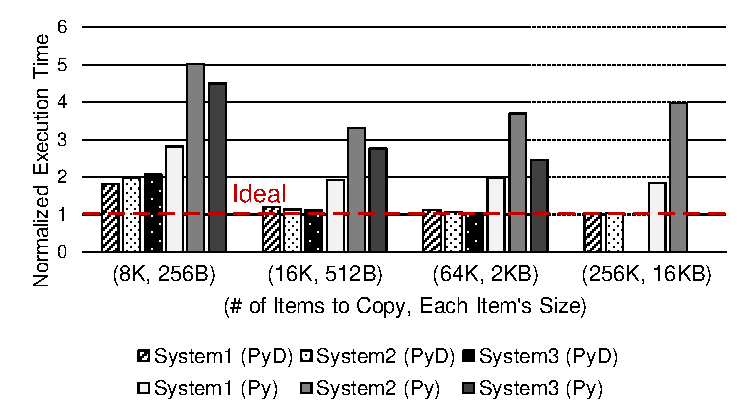
\includegraphics[width=0.85\linewidth]{figures/PyDArXiv/microbench_vs.pdf}
    \caption{Irregular host data access pattern microbenchmark comparisons between PyTorch (Py) and PyTorch-Direct (PyD) on different systems. The ideal case shows only the pure data transfer time with a peak PCIe bandwidth.}
    \label{fig:micro_fig}
\end{figure}
\begin{figure}[]
    \centering
    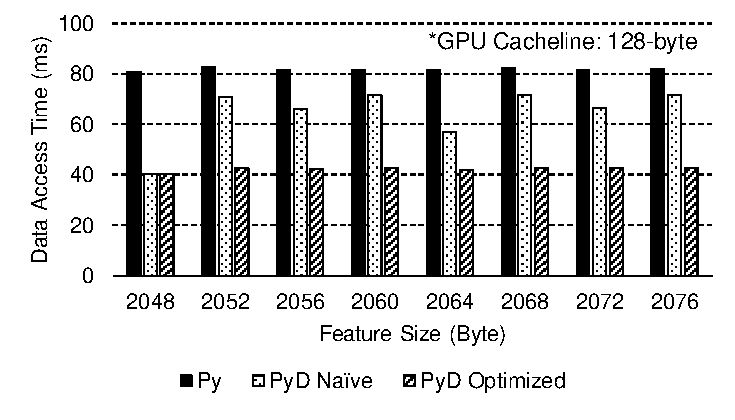
\includegraphics[width=0.85\linewidth]{figures/PyDArXiv/alignment.pdf}
    \caption{Memory access alignment and its impact on PyTorch-Direct (PyD) performance. PyTorch (Py) results were added for comparison.}
    \label{fig:alignment}
\end{figure}

To evaluate the impact of the memory alignment optimization in PyTorch-Direct, we measure data access times for various feature sizes from 2048-byte to 2076-byte in a 4-byte stride.
The result is shown in Figure~\ref{fig:alignment}.
For the \texttt{PyD Naïve} case, we use the unmodified GPU indexing kernel from PyTorch, and the kernel has no knowledge of memory alignment.
For the \texttt{PyD Optimized} case, the optimization from Section~\ref{sec.PyTorch_direct.implementation.alignment} is applied.

Figure~\ref{fig:alignment} shows that PyTorch-Direct reduces the data access time significantly compared to the PyTorch baseline.
However, the benefit is limited without the memory-alignment optimization.
For example, when the feature size is 2052 bytes, the \texttt{PyD Naïve}  provides only 1.17$\times$ of performance improvement over \texttt{Py}, while the \texttt{PyD Optimized} provides 1.95$\times$ of performance improvement.
Based on the results, we observe the optimization provides a consistent benefit over the PyTorch baseline (averagely 1.93$\times$) regardless of the data alignment.


\subsection{GNN Training Performance}


\begin{figure}[!htbp]\captionsetup[subfigure]{font=small}
\centering
\subcaptionbox{GraphSAGE}
[\linewidth]{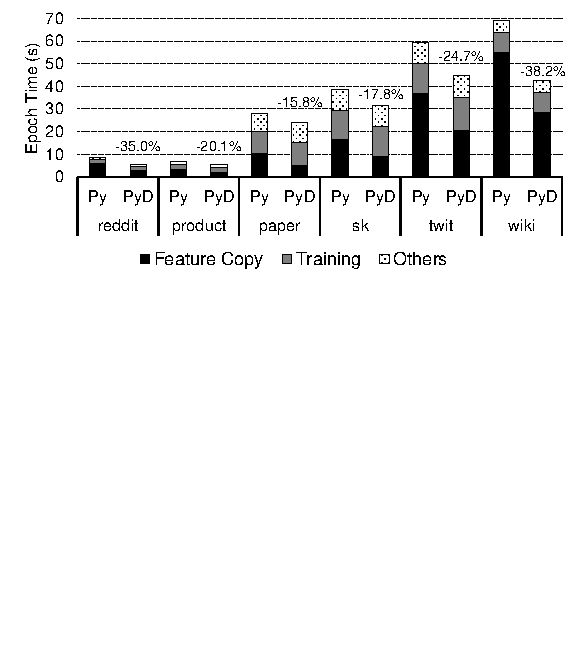
\includegraphics[scale=1.2]{figures/PyDArXiv/combined_perf_graphsage.pdf}}
\subcaptionbox{GAT}
[\linewidth]{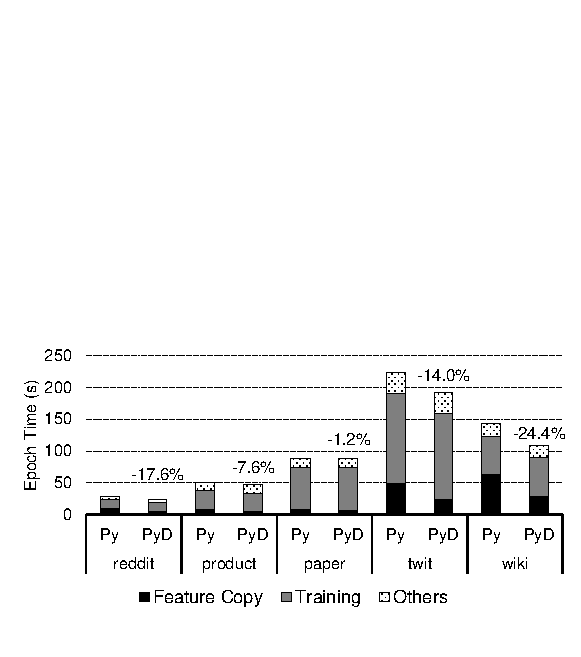
\includegraphics[scale=1.2]{figures/PyDArXiv/combined_perf_gat.pdf}}
\caption{\label{fig:graphsage} Single epoch execution time breakdown for both PyTorch (Py) vs. PyTorch-Direct (PyD) when running (a) GraphSAGE and (b) GAT in different datasets. Training epoch time reductions are written on the bars.}
\end{figure}


In Figure~\ref{fig:graphsage}, we compare the breakdown of the training epoch time when using unmodified DGL implementations in PyTorch vs. PyTorch-Direct.
In the GAT training, we do not run \texttt{sk} dataset due to the DGL's out-of-host-memory error for both PyTorch and PyTorch-Direct cases.
Similar to the microbenchmark results in Section~\ref{sec.evaluation.microbenchmarkI}, we observe about 47.1\% reduction in the feature copy times.
The other portions of the training epoch times remain almost identical to the baseline case.
PyTorch-Direct gives less benefit for datasets with smaller feature sizes (e.g., \texttt{paper}) because the feature copy time is smaller in the end-to-end training time.
Similarly, GAT training is computationally heavier than GraphSAGE, and therefore, we observe less benefit of PyTorch-Direct.
Overall, we observe between 1.01$\times$ to 1.45$\times$ speedup when we use PyTorch-Direct in GNN training.
